\documentclass[12pt,oneside]{report}

% ---------- Packages ----------
\usepackage[utf8]{inputenc}
\usepackage[T1]{fontenc}
\usepackage{lmodern}
\usepackage{setspace}
\usepackage{geometry}
\geometry{letterpaper, margin=1in}
\usepackage{graphicx}
\graphicspath{{figures/}}
\usepackage{caption}
\usepackage{subcaption}
\usepackage{booktabs}
\usepackage{amsmath, amssymb}
\usepackage[hidelinks]{hyperref}
\usepackage[nameinlink,capitalise]{cleveref}
\usepackage{enumitem}
\usepackage{xcolor}
\usepackage{titlesec}
\usepackage[T1]{fontenc}
\usepackage{lmodern}
\usepackage{xparse}

% Minimal approach - let LaTeX handle TOC normally
\usepackage{csquotes}
\usepackage[style=numeric,natbib=true,sorting=none]{biblatex}


\NewDocumentCommand{\scsurname}{m m o}{%
  #1~\textsc{#2}%
  \IfValueT{#3}{\space #3}%
}

\addbibresource{references.bib}

\setcounter{secnumdepth}{3}
\setcounter{tocdepth}{2}
\onehalfspacing

% Custom chapter formatting - remove "Chapter" prefix and newlines
\titleformat{\chapter}[hang]
{\normalfont\Large\bfseries}{\thechapter}{1em}{}
\titlespacing*{\chapter}{0pt}{0pt}{20pt}

% ---------- Convenience ----------
\newcommand{\todo}[1]{\textcolor{red}{TODO: #1}}

% ---------- Title Info ----------
\newcommand{\proposaltitle}{Deep Learning for Scalable Sensorimotor Brain-Computer Interfaces}
\newcommand{\authorname}{Joel Ye}
\newcommand{\department}{
  Neural Computation, Neuroscience Institute \\
  Machine Learning Department, School of Computer Science \\
}
\newcommand{\university}{Carnegie Mellon University \\ Pittsburgh, PA}
\newcommand{\proposaldate}{July 30, 2025}

\newcommand{\committee}{%
  \scsurname{Robert}{Gaunt}[({co-chair})]\\[0.15\baselineskip]
  \scsurname{Leila}{Wehbe}[({co-chair})]\\[0.15\baselineskip]
  \scsurname{Jennifer}{Collinger}\\[0.15\baselineskip]
  \scsurname{Aran}{Nayebi}\\[0.15\baselineskip]
  \scsurname{Chethan}{Pandarinath}[({Emory University})]%
}

% ---------- Document ----------
\begin{document}

% --- title page ---
\begin{titlepage}
\setlength{\parindent}{0pt}
\centering

% top breathing room
\vspace*{\stretch{1}}

% Title block
{\LARGE\bfseries \proposaltitle\par}
\vspace{0.6\baselineskip}
{\Large \authorname\par}

\vspace{1.5\baselineskip}
{\large PhD Thesis Proposal\par}
{\small \proposaldate\par}

\vspace{1.2\baselineskip}
{\normalsize
\begin{minipage}{0.9\textwidth}\centering
\department
\university
\end{minipage}\par}

% middle breathing room (larger to push committee lower)
\vspace*{\stretch{2}}

% Committee block
{\large\bfseries Thesis Committee:\par}
\vspace{0.4\baselineskip}
{\normalsize
\begin{minipage}{0.7\textwidth}\centering
\setlength{\parskip}{0pt}%
\committee
\end{minipage}\par}

% bottom breathing room (largest to anchor footer)
\vspace*{\stretch{3}}

{\small\itshape
Submitted in partial fulfillment of the requirements for the Degree of Doctor of Philosophy\par}

\vspace*{\stretch{1}}
\end{titlepage}
\pagenumbering{arabic}

\section*{Abstract}
\addcontentsline{toc}{section}{Abstract}
The increasing ambition of neuroscience and neurotechnology both supplies and demands vast new quantities of neural data, which creates a critical need for methods that can operate effectively on neural data at scale.
This need could potentially be addressed by deep learning (DL).
Here, we assess this program for sensorimotor intracortical brain-computer interfaces (iBCI). iBCI systems have traditionally been built by collecting short datasets to relate a user’s neural activity with their bodily state. Although this approach can enable both motor control and sensory feedback in research settings, iBCI's real-world adoption will further depend on achieving high performance with exquisite reliability and convenience. In other words, iBCI systems must too, evolve to operate effectively on BCI data at real-world scales.
To this end, I present one completed study and two proposed projects that show how deep learning models can provide a platform for scaling BCI systems. Through this platform, I promote a view that BCI models can and should be built to reflect the BCI system's lifelong data collection.

% Therefore, this challenge might be best met with deep learning models that encapsulate the landscape of data accumulated throughout the BCI device's lifetime.
% Therefore, this challenge might be best met with deep learning models that encapsulate the landscape of data accumulated throughout the BCI device's lifetime.
% deep learning becomes an  provide a tractable platform with which to encapsulate this landscape.
% That is, by reframing the accumulation of BCI datasets throughout device lifetime not as standalone snapshots but as a landscape of related data,
%  reframe BCI data not as a collection of standalone datasets but as a store of related data accumulated throughout the BCI device's lifetime.
% I next introduce one result and two proposed works that build this case.

\textbf{Aim 1: Large scale pretraining improves modeling of intracortical motor datasets [in submission].}

The driver of deep learning’s efficacy across domains is its ability to leverage conserved statistical structure across datasets, primarily enabled by a stage of model preparation on large scale data called pretraining. Previous work has identified the requisite conserved structures across motor cortical datasets, and so we systematically measure the efficacy of deep neural network (DNN) pretraining on such datasets. We establish that DNN efficacy improves with neural data scale on both multi-subject and multi-behavior datasets. Yet, this scaling has diminishing returns as data in the downstream, target setting grows, rendering the scaling less impactful for long term BCI applications. We conclude that pretrained networks may accelerate initial BCI calibration speeds but will not fundamentally remove the need for continuous BCI data collection.

\textbf{Aim 2: Pretrained deep networks enable rapid and scaleable upper limb neuroprosthetic control [proposed].}

High degree of freedom control of a robotic arm and hand is possible with current iBCIs, but requires extensive daily recalibration and experimenter intervention. Based on successful deep network use in speech BCIs, we propose that an NDT-based controller (NDT3o) which accumulates calibration data across days can address both of these challenges. We will evaluate NDT3o for 7-degree of freedom neuroprosthetic arm and hand control in up to two human participants, aiming to demonstrate continuous high performance in functional tasks of robotic upper limb control. We further aim to demonstrate the model’s scalability by extending this control to additional degrees of freedom in the hand without changes to the model design.

\textbf{Aim 3: Modeling intracortical microstimulation for sensory BCIs [proposed].}

Sensory feedback is integral to native motor control, and can be provided in iBCIs through intracortical microstimulation (ICMS) of the somatosensory cortex. The sensory feedback provided by ICMS has been shown to improve BCI control, but our understanding of how ICMS accomplishes this through its modulation of ongoing neural activity is poor. Specifically, we lack a predictive model of the neural response to ICMS, which stunts the development of any sophisticated ICMS protocols. Towards this goal, we first introduce a method to recover spiking activity from artifacted recordings, and then taxonomize the sensory neural response to ICMS through DNN transfer learning experiments. In this taxonomy, we show that while deep networks largely generalize to temporal variety in stimulation patterns, they fail to generalize to new stimulation channels. These results inform the development of stimulation protocols to accurately map the neural response to ICMS.

% Table of contents
\tableofcontents

\cleardoublepage
\pagenumbering{arabic}

% =========================
% Introduction
% =========================
\chapter{Introduction and Background}

\begin{figure}[h]
  \centering
  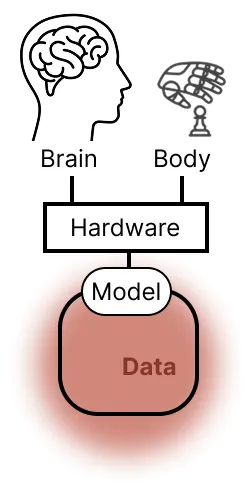
\includegraphics[width=0.3\linewidth]{ch1_bci_schema.png}
  \caption{The role of a computational model is to provide an interface to interact with the underlying domain data. A scalable model is one that provides a tractable strategy to encapsulate and query a growing variety of data.}
  \label{fig:bci_schema}
\end{figure}

Today, neuroscientists seek to study the brain in natural, dynamic environments, and neurotechnology companies are similarly racing to produce a device that will work robustly in the real world. In this increasing scope, modeling neural data begins to resemble a problem of a thousand cuts.

Because we are not mechanistic, we must observe and hope the rules that govern the system we observe in situations that we can tractably analyze ... hold in broader situations. Naturally, any number of factors can break this down, and indeed, break down it does.

Radically empiricist data-driven....

Today, neuroscientists seek to study the brain in natural, dynamic environments, and neurotechnology companies are similarly racing to produce a device that would work robustly in the real world. The challenge of modeling even a fraction of the brain within this broad scope resists specific definition because it is a problem of a thousand cuts. The neural data we study in iBCIs, namely the spiking activity of single neurons in tiny volumes of human cortex, are affected by innumerable factors. These factors stem from the fact that the recorded neurons are nestled in a highly interconnected biological network that changes on many timescales, and their activity only arrives to our models only after passing through several layers of BCI hardware and software. When these factors are stable, the connection between neural data and behavior can appear remarkably straightforward, motivating the use of simple and interpretable models. However, when these factors shift, unobserved to us, the performance of our models can quickly degrade. Regardless of one’s philosophy on whether we can exhaustively characterize these factors and ultimately understand the data we collect, we undoubtedly should expect to continuously evaluate and update our models as we expand the scope of their application. To minimize the Sisyphean burden of this task, many domains faced with similar challenges have turned to deep neural networks, deprioritizing interpretable theories in favor of a data-centric view of modeling, where the role of the model is merely to capture and interface with the underlying domain data. % ~\figref{fig:schema}.

In this proposal, I aim to establish such a data-driven framework for thinking about sensorimotor BCIs, describing three ways in which we can use deep networks to relate and aggregate BCI datasets. To contextualize this work, I will introduce brain computer interfaces and deep learning’s application to BCIs in turn.

TODO define figref.

\section{Brain-computer interface models}
\begin{figure}[h]
  \centering
  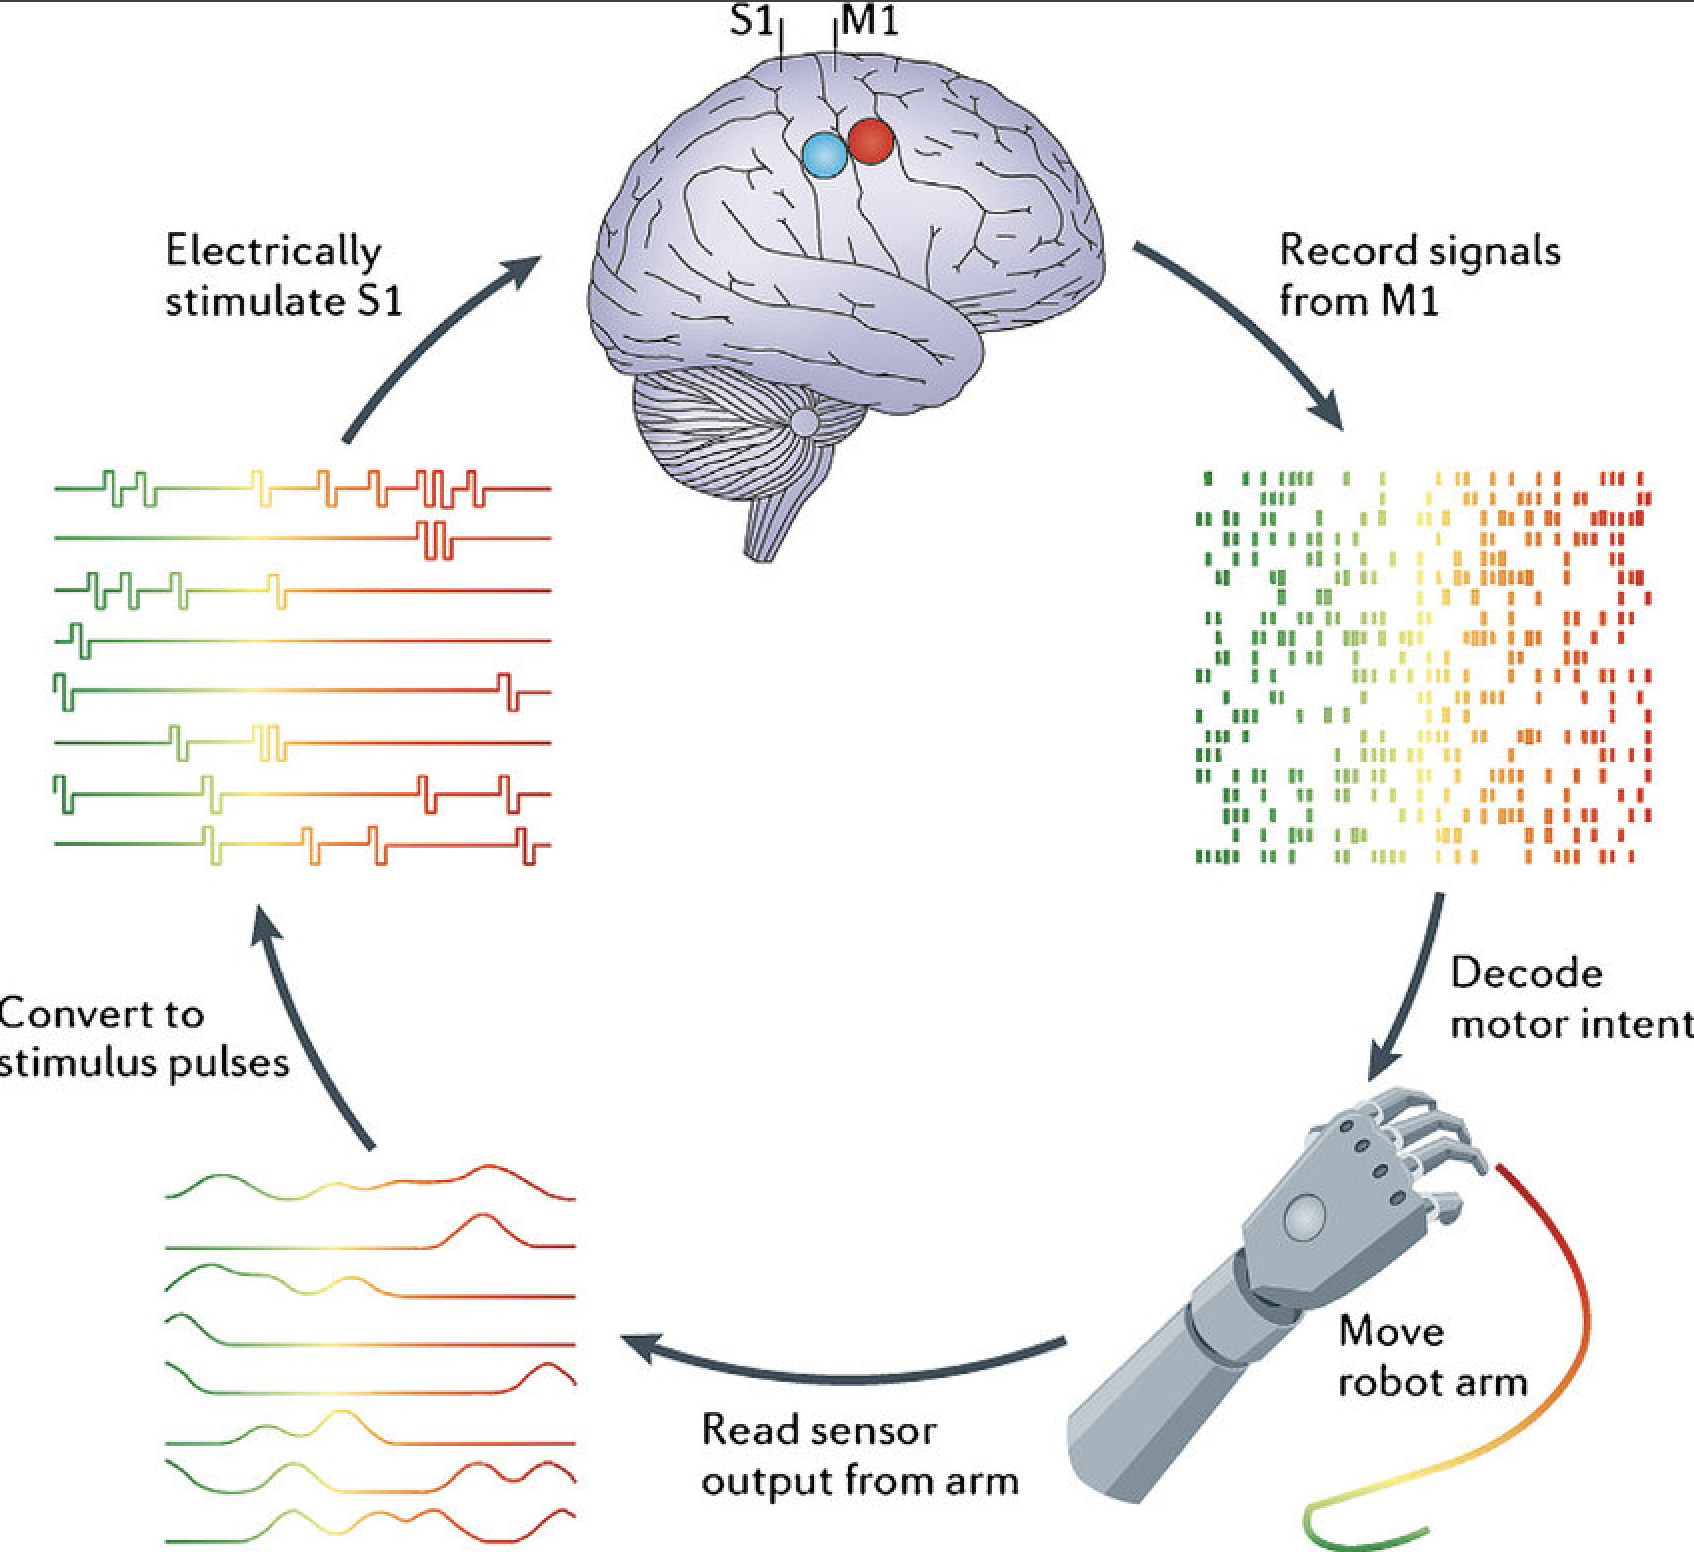
\includegraphics[width=0.5\linewidth]{ch1_bci_loop.png}
  \caption{Brain-computer interface control loop.}
  \label{fig:bci_loop}
\end{figure}

A brain-computer interface (BCI) is a system that allows observation and control of neural activity. In the rehabilitative setting, BCIs mainly observe motor cortex to predict movement intentions and control sensory cortex to evoke sensations. By modeling the relationships between these variables, the sensorimotor BCI aims to provide a degree of sensorimotor function and independence for the paralyzed user.

Over the last two decades, a number of studies have demonstrated the efficacy of human BCIs based on implanted microelectrode arrays (Blackrock Utah arrays). With implants in motor cortex recording neuronal spiking activity, users have achieved control of digital cursors, robotic arms, and language and speech generation~\citep{pandarinath2017high,collinger2013high,willett_21_handwriting,willett_23_speech}. With stimulation of implants in somatosensory cortex, users perceive tactile sensations on their hand that is valuable as an end in itself [values survey, first sensation papers] and can also be utilized functionally for more skillful motor control [flesher and other sensation refs]. The main agendas for BCI algorithms research are to make this existing repertoire more robust and performant, to develop new BCI capabilities, and to deploy convenient systems to users with reduced need for calibration [chethan’s survey?].

To illustrate directions for progress in motor BCIs, we schematize the timeline of BCI performance in [Fig]. Standard BCI models must be initialized with a calibration protocol where experimenters collect by paired neural activity and motor intention labels by prompting the user to behave according to experimental cues. The black arc shows how BCI performance will increase with this calibration period [Makin], but then decline over time due to signal nonstationarities that render the calibration data less relevant [nonstationarity refs]. The burden of the calibration period can be reduced by improving our model priors, and performance can also be preserved through varied recalibration strategies. This model has been executed well by speech BCIs [Willett, Card, Fan]. There, hundreds of calibration sentences are collected on the timescale of an hour, to calibrate an initial language decoder. This decoder provides a powerful enough prior that high performance decoding can be achieved in subsequent BCI sessions with only a few new calibration sentences. As time passes and decoding errors begin to increase, an external language model can provide the weak learning signal needed to maintain high performance decoding for months. A comparably stable and high performance BCI for upper limb control remains to be demonstrated.

Current somsatosensory BCIs are in a pre-paradigmatic state. Plainly, there is no strongly predictive model of what different intracortical microstimulation (ICMS) patterns will do in a particular individual or implant, so the analogous calibration process is to collect perceptual reports as many different stimuli as fit within experimental time constraints. The most studied parameterization of ICMS is under fixed frequency and amplitude pulse trains on single electrodes. Under this parameterization, the evoked sensation is highly stable over time, but the precise quality and intensity of the sensation can vary across days [citation needed]. Worse, the impacts of stimulation frequency and amplitude on these sensations will vary across stimulation electrodes [Hughes]. One promising development towards more precise and reliable ICMS is the principle of biomimicry. Biomimetic ICMS motivates the design of stimulation pulses evoke neural responses resembling those of natural touch, rather than the merely convenient design space of fixed frequency and amplitude pulse trains. However, this aspiration is hamstringed on both ends, as it is difficult both to observe the neural response to ICMS and to observe the neural response to natural touch in BCI participants who typically have impaired somatosensory pathways. Current demonstrations of biomimetic ICMS have compromised by matching coarse, subject-general features of natural touch and assuming the neural response to ICMS is proportional to either frequency or amplitude inputs. Realizing biomimetic ICMS in higher fidelity through local neural activity, and thereby presumably improving somatosensory BCI efficacy overall, will require addressing both these assumptions.

\begin{figure}[h]
  \centering
  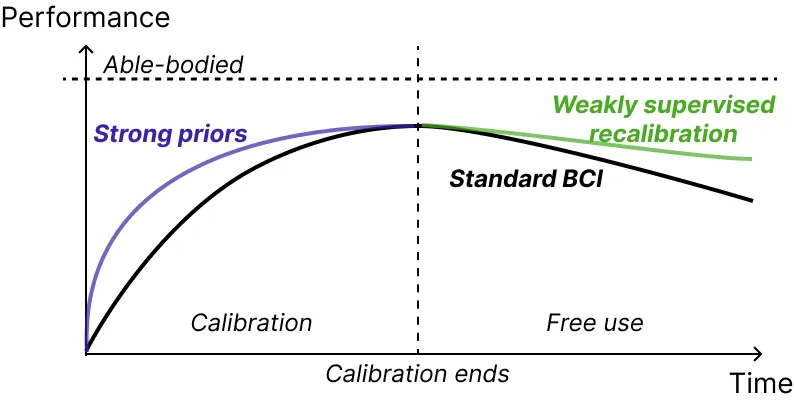
\includegraphics[width=0.5\linewidth]{ch1_ibci_stability.png}
  \caption{iBCI stability challenges.}
  \label{fig:ibci_stability}
\end{figure}

Current somatosensory BCIs are in a pre-paradigmatic state. Plainly, there is no strongly predictive model of what different ICMS patterns will do in a particular individual or implant, so the analogous calibration process is to collect perceptual reports for as many different stimuli as fit within experimental time constraints. The most studied parameterization of ICMS is under fixed-frequency and fixed-amplitude pulse trains on single electrodes. Under this parameterization, the evoked sensation is highly stable over time, but the precise quality and intensity of the sensation can vary across days \citep{citationNeeded}. Worse, the impacts of stimulation frequency and amplitude on these sensations will vary across stimulation electrodes \citep{hughesPlaceholder}. One promising development towards more precise and reliable ICMS is the principle of biomimicry, which motivates the design of stimulation pulses that evoke neural responses resembling those of natural touch. Realizing biomimetic ICMS in higher fidelity through local neural activity will require addressing assumptions on both the neural and perceptual sides.

\section{Deep network models of BCI data}

Modern deep learning organizes applications research by the data being modeled, the model architecture, and the optimization objective. We will take this approach to introduce deep networks in BCI.

\textbf{Data}: The neural data recorded from our BCIs are multichannel voltage timeseries. Most traditionally, and in the majority of this proposal, this broadband voltage will first be filtered and thresholded to extract rapid, transient deflections, which putatively reflect a spike on a neuron nearby the recording electrode. A typical BCI dataset will include 100 to 200 electrode channels of data with dozens of clearly indicated neurons, along with many more channels with neural “hash” where nondistinctive spiking waveforms dominate. Our motor datasets will also contain upper limb covariates, for example in the form of kinematics or electromyography that varies on the timescale of seconds. In non-human primate datasets, these behaviors generally derive from physical sensors, but a different strategy must be used to create human BCI datasets since human BCI users have impaired control of their native limb. Human BCI datasets instead assert a certain behavior and experimentally cue the user to attempt the behavior. This artificial association means that the behavior label is likely to be temporally warped and otherwise imprecise~\citep{merel2016neuroprosthetic} relative to the unobserved motor intention of the user. We can also frame this process as a user labeling of the cued behavior data with their neural activity. The electrical stimuli that we use in sensory datasets comprise trains of biphasic current-controlled pulses, where each individual pulse’s timing and amplitude can be varied. Perceptual reports to ICMS, to the extent we will mention in this proposal, will be described in terms of binary detection or scalar ratings.

\textbf{Architecture}: The mainstays of broader deep learning architectures that have flourished in the last decade, including MLPs~\citep{Willsey2022HighVelocity}, convolutional neural networks (CNNs)~\citep{temmar2024artificial}, recurrent neural networks (RNNs)~\citep{pandarinath_18_lfads}, and Transformers~\citep{ye_21_ndt}, have all been applied to BCI data. Unlike in other domains, BCI has yet to provide any decisive verdict on the most performant architectures. This proposal presumes the view of the Bitter Lesson~\citep{sutton2019}, and presumes that performance differences across architecture may ultimately be less robust than gains from increasing data scale. Adopting this view, we will mainly distinguish two superordinate model classes, the RNN and the Transformer. RNNs process timeseries data one timestep at a time, maintaining an internal state that evolves with the input data. An RNN provides an appealing interpretation for neural data, as its weights describe the evolution of the neural dynamical system. The Transformer, in contrast, does not maintain a centralized state but instead learns the relationship between fragments of the data. Each of these fragments is called a token, and they could be for example the population activity vector at the start of an experimental trial, abstract metadata about the experiment, or the vertical velocity of a user’s arm. Transformers feature widely in this proposal due to their empirical dominance across machine learning (ML) domains, including even other timeseries domains like audio processing~\citep{radford2022whisper}.

\textbf{Objective}: The objectives used in this proposal all fall under prediction, whether regression or classification. This will be true despite the fact that different models may have qualitatively different functions. When the work’s objective is to model neural data in isolation, we are interested in the model’s representation learning. At other times, we say we are building decoders of neural data to predict behavior, or encoders of stimuli to predict neural activity. With the lens of deep networks in particular, these different terms all implementationally overlap, in that the underlying models are operating between one or two data modalities.

\textbf{Challenges}: BCI datasets feature a number of challenges that uniquely interact with deep learning. First, by experimental design, there is often a large component of the neural data that appears strongly connected to the covariate of interest, implying there is not an immediately clear role for nonlinear DNNs. For example, in the motor cortex, we can identify single neurons with firing activity that can be well characterized by a cosine tuning curve with two parameters, a preferred arm direction and depth of firing rate modulation to movement in that direction. To balance this simplicity, BCI datasets will often have nonstationarities~\citep{downey_18_stability,wimalasena2020unstable,perge2013intra}. New cognitive states, neurophysiological changes at the electrode interface, and BCI system hardware state can all introduce shifts in the observed activity. These externalities are difficult to directly observe, so we must build systems that are implicitly robust to these shifts so as to enable stable BCI performance~\citep{sussillo_16_future}.

A modern aspiration of deep networks is their ability to provide broad performance gains on tasks in a field, once trained on sufficiently broad data within said field. Once a model is designated as having this general capability, it is given the somewhat aspirational title of a foundation model. Foundation models were most deservingly coined in the context of natural language processing (NLP), where large scale training created a model that quickly dominated all mainstream benchmarks. Critically, model performance gain correlates reliably with the scale of initial training, or pretraining, providing the impetus for many fields to aim to measure the empirical “scaling” of model performance with data. A contingent of neuroscientists now seeks to establish a similar paradigm for neural data, by amassing large neural data repositories and performing similarly scaled model training~\citep{dyerSOMETHING}. Aim 1 performs precisely this effort for BCI data.

\textbf{Deep learning as systems tools}: The practice of deep learning is distinguished from the broader machine learning discipline by its empirical culture. Mantras on model behavior develop based on what has previously been effective, like focusing on data over models or focusing on broad task performance over single tasks~\citep{abnar2021exploringlimitslargescale}. One pertinent empirical view is that foundation models are at minimum a catalog of their training data, and can easily learn simple functions. The value of this capability is exemplified in text cleaning, a domain that systems researcher Christopher Ré describes as facing a death by a thousand cuts, where individual problems are not technically challenging but their breadth and non-enumerability frustrate systematic solutions. Remarkably, early language models (GPT3) provided a simple solution to sanitizing human text entry and documents for errant values, outperforming rules-based agglomerations that received years of investment. Similarly, neural data appears locally linear in any given context, and the neural population activity may in fact be neatly organized so that certain aforementioned nonstationarities may simply not degrade existing models. It would be foolhardy to expect this in generality, however, as simply across behaviors, the neural data distribution will begin appearing nonlinear~\citep{fortunato2024nonlinear}. It is thus through this systems lens that I most expect BCIs to benefit from deep learning.

\section{Summary}



% =========================
% Aim 1
% =========================
\chapter{Aim 1: Large-scale pretraining for intracortical neural datasets}

\section{Summary and Significance}
Deep learning’s greatest successes have depended on exploiting large and varied datasets. We perform two scaling studies on Transformer pretraining for motor cortical decoding, measuring returns on increased pretraining across sessions, subjects, and tasks. Cross-session data scales nearly as well as same-day data, while cross-subject and cross-task data yield positive but attenuated returns. Pretraining on $\sim$2000 hours of pooled activity continues to help, but benefits decline rapidly as downstream data grows (converging near $\sim$90 minutes of task data). Thus, pretraining accelerates calibration but does not eliminate the need for ongoing data collection.

\paragraph{Papers.} Ye et~al., ``Neural Data Transformer 2''; Ye et~al., ``A Generalist Intracortical Motor Decoder.''

\section{Approach}
We study pretraining (large, loosely related datasets) and fine-tuning (small, closely related data) while varying data volume, diversity, model size, and compute. Evaluation uses fixed held-out contiguous blocks per dataset. The NDT2 and NDT3 architectures tokenize spikes in 20\,ms bins and spatial patches; NDT2 follows a masked prediction objective, while NDT3 is autoregressive and supports variable behavioral dimensionality.

\begin{figure}[h]
  \centering
  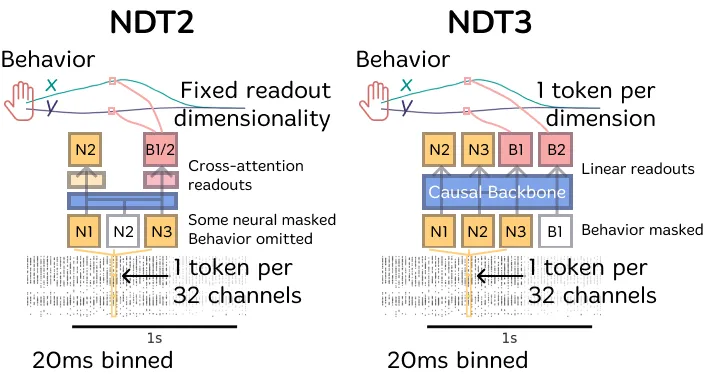
\includegraphics[width=0.5\linewidth]{ch2_ndt_models.png}
  \caption{NDT2 and NDT3 both take input neural data and output neural data and behavior predictions. Both models tokenize neural data in time with 20ms timebins and in space by dividing the population activity into subsets of fixed size (32 in this figure). NDT2 emits one behavior token for prediction at each timestep, while NDT3 emits one behavior token per behavior dimension and timestep, which enables streamlined prediction of behavioral data of varied dimensionality. NDT2, inspired by a Masked Autoencoder design [He], masks out a fraction of neural token inputs and only predicts this fraction. NDT3 adopts the autoregressive modeling framework and allows prediction of all neural tokens conditioned on neural tokens from previous timesteps.}
  \label{fig:ndt_models}
\end{figure}

\section{Results}
NDT2 demonstrates transfer across sessions/subjects/tasks via population patching, Pareto-dominating from-scratch models in zero-shot and with small supervised/unsupervised calibration. NDT3 scales pretraining to 2000\,h and confirms: (i) pretraining helps broadly up to $\sim$90\,min of downstream data, after which from-scratch models catch up; (ii) larger pretraining datasets and models yield better averages.

\begin{figure}[h]
  \centering
  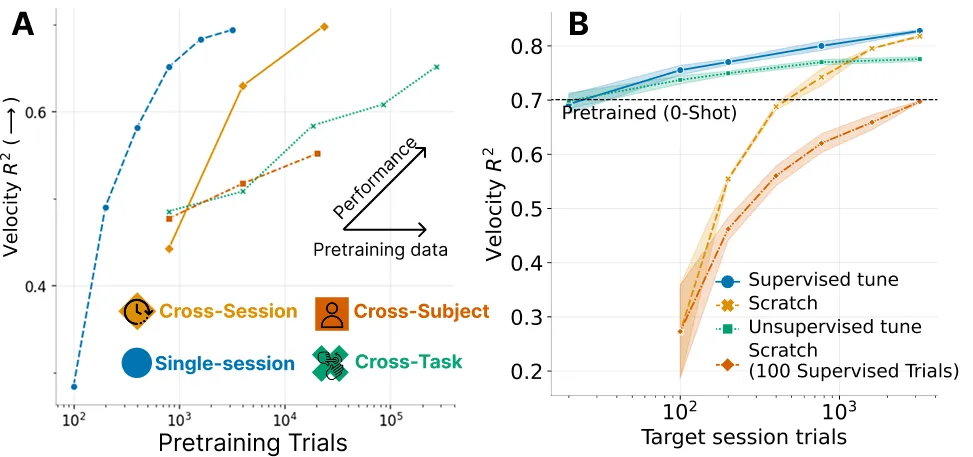
\includegraphics[width=0.5\linewidth]{ch2_ndt2_results.png}
  \caption{A. NDT2 decoding of monkey reach velocity scales with increasing pretraining data from different sessions, subjects, and behavioral tasks. The pretraining abscissa for the single-session curve indicates the total training data available to the model. For the order curves, the abscissa indicates the pretraining data scale. These pretrained models fine-tune to the target session with 100 trials of data. B. Pretrained multisession models can be deployed on new sessions for immediate zero-shot performance. They can also be tuned either through supervised or unsupervised objectives to improve performance, which pareto-dominates performance achieved by training models from scratch.}
  \label{fig:ndt2_results}
\end{figure}

\begin{figure}[h]
  \centering
  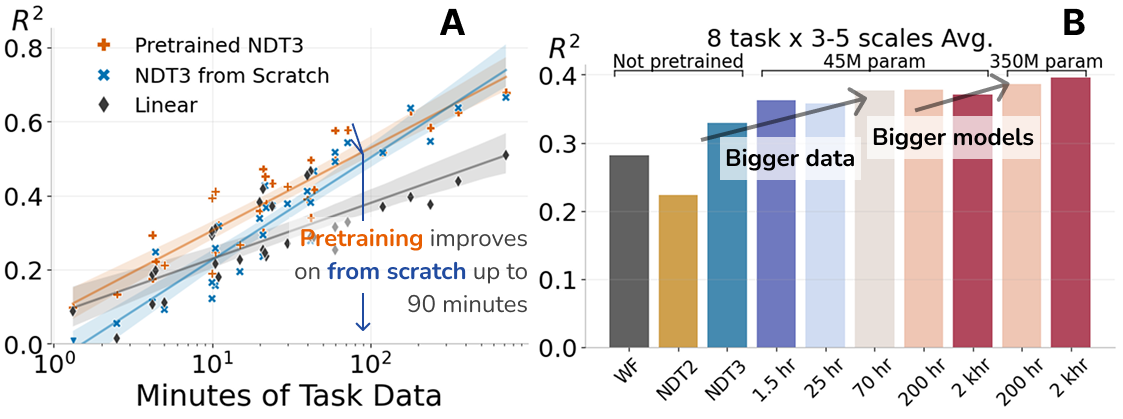
\includegraphics[width=0.5\linewidth]{ch2_ndt3_summary.png}
  \caption{Two summary views of all evaluations conducted on NDT3 models. Left: When evaluations are organized by downstream data scale (Minutes of Task Data), a pretrained model is better than or equal to non-pretrained models and a linear baseline at all data scales. However, the non-pretrained NDT3 model matches the pretrained model when downstream task data is sufficiently large, here at 90 minutes. Right: Collapsing all evaluations into a single average, we see that scaling pretraining dataset size and model size improves summary performance.}
  \label{fig:ndt3_summary}
\end{figure}

\begin{figure}[h]
  \centering
  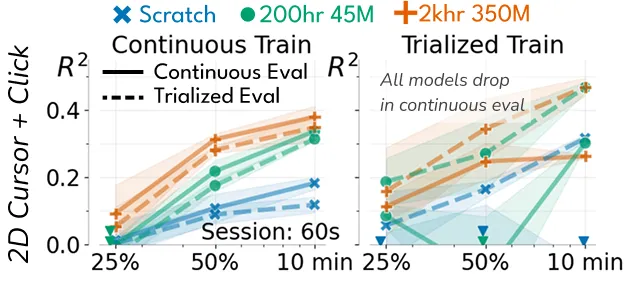
\includegraphics[width=0.5\linewidth]{ch2_trialized.png}
  \caption{Models are evaluated on a human open-loop cursor dataset prepared in two ways. Trialized training receives inputs according to trial boundaries, varying from 2-4 seconds in length. Continuous training receives random 1 second snippets (that can cross trial boundaries). Trialized evaluation matches trialized training, and continuous evaluation is done by streaming up to 1 second of history. Downward arrows indicate points below 0.0. Continuously trained models perform well in both evaluation settings, while models trained on trialized data fail in continuous evaluation.}
  \label{fig:trialized}
\end{figure}

% =========================
% Aim 2
% =========================
\chapter{Aim 2: Pretrained deep networks enable continuous and scalable upper-limb neuroprosthetic control}

\section{Summary and Significance}
Implanted BCIs can decode diverse upper-limb behaviors, but current decoders need substantial daily calibration and underperform able-bodied control. We propose NDT3-based controllers accumulating calibration across days to deliver robust 7--9\,DoF control in up to two participants, and to demonstrate scalability to additional hand DoF without architectural changes.

\section{Approach}
Key ideas: (i) shift from daily retraining to a large initial calibration plus brief daily adaptation; (ii) extend to higher DoF, starting with thumb and grouped fingers. Calibration uses virtual reach--grasp--carry sequences at multiple speeds; training uses robust objectives (e.g., Soft-DTW). Evaluation includes ARAT and timed object transfer, plus virtual metrics (path efficiency, phase-wise performance).

\section{Results \& Remaining Work}
Pilots: NDT3 matches linear decoders for 2D cursor control; ReFIT improves linear speed more than NDT, suggesting gain/label-noise sensitivity. In 4D Mujoco control, linear decoders degrade under unconstrained DoF due to instability, whereas NDT maintains performance via implicit DoF isolation. Multiday adaptation boosts success and completion time, supporting feasibility for continuous 7D control.

\begin{figure}[h]
  \centering
  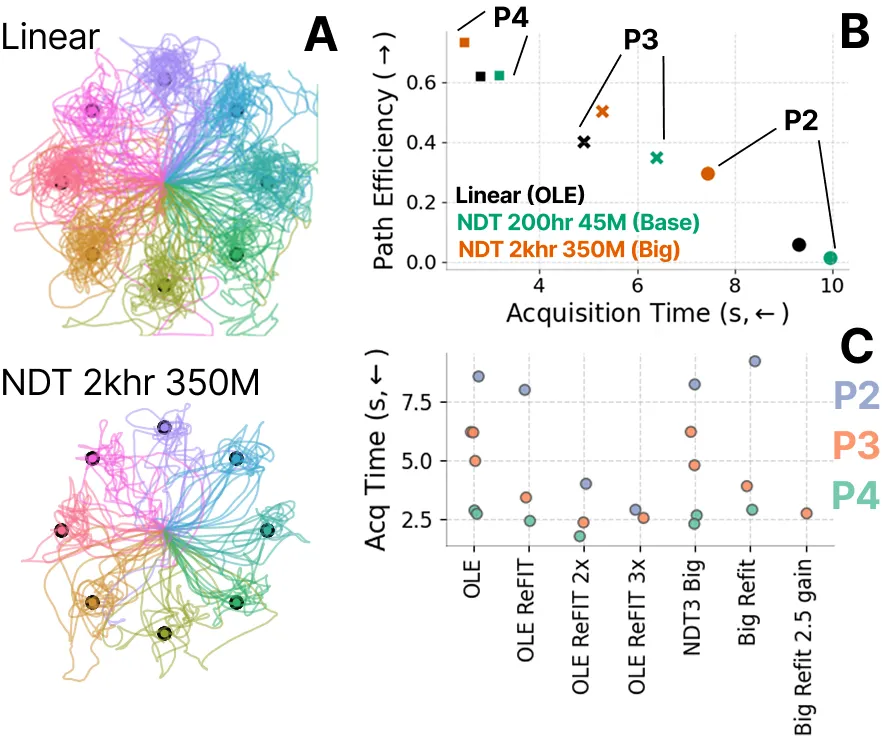
\includegraphics[width=0.5\linewidth]{ch3_cursor_control.png}
  \caption{A. OLE and NDT brain-control trajectories in one human participant. B. NDT matches linear model performance for 2D cursor control when all models are trained on an open loop calibration block. Fitting the large NDT model is preferred. B. After closed loop tuning, linear control steadily improves, but NDT speed does not. Gain can be increased to keep NDT at pace.}
  \label{fig:cursor}
\end{figure}

\begin{figure}[h]
  \centering
  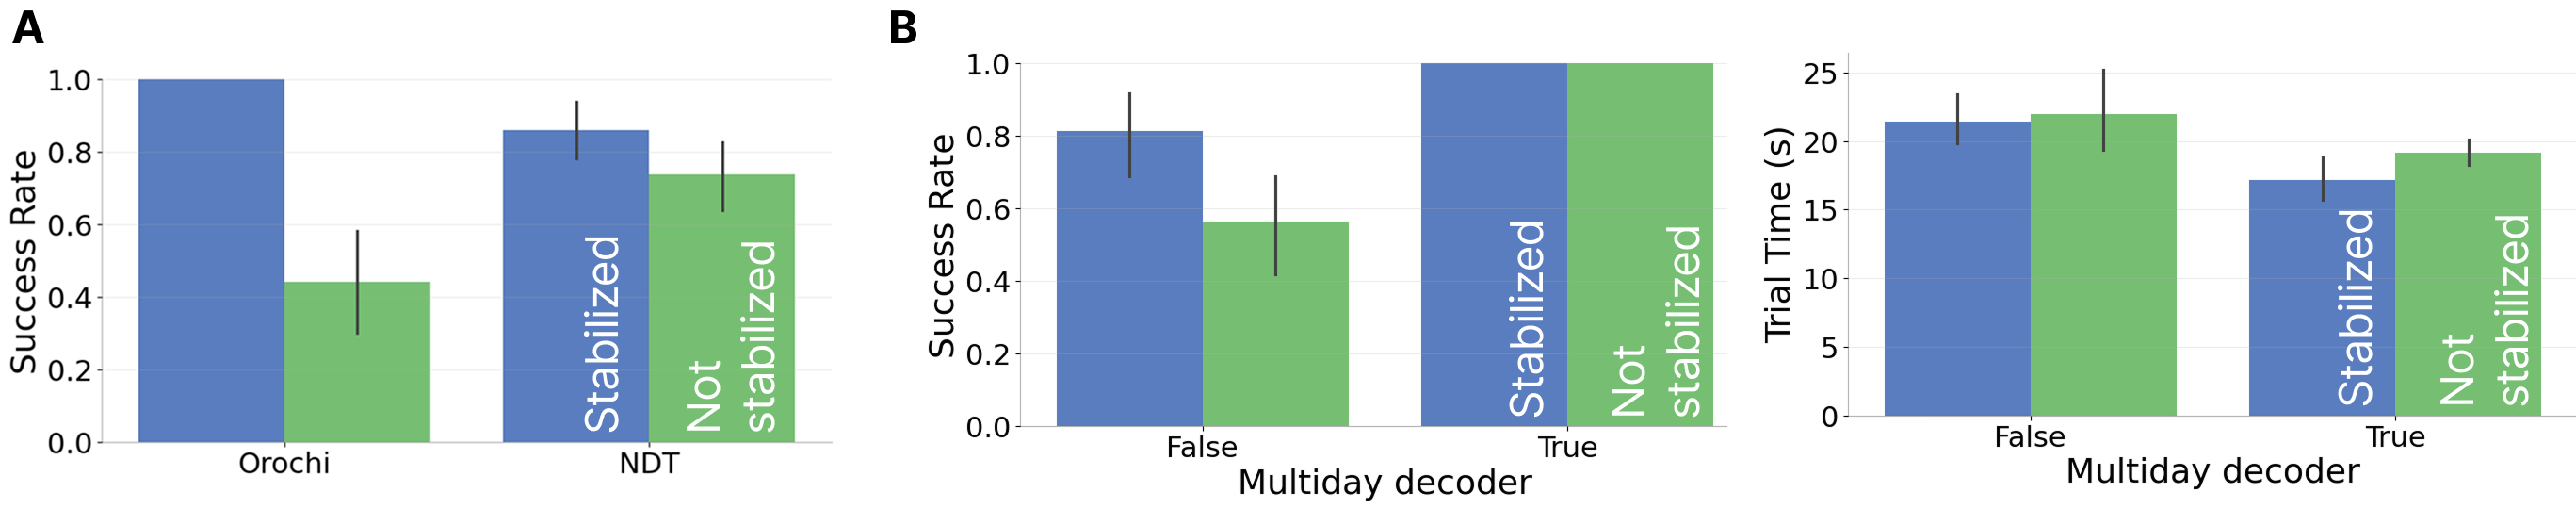
\includegraphics[width=0.5\linewidth]{ch3_mujoco_results.png}
  \caption{A. Orochi linear decoder compared against NDT DNN decoder for Mujoco 4D FBC Sequenced movement trials. Error bars show standard deviation across trials. Evaluations are conducted in constrained and unconstarined settings. Constrained evaluations only allow one of arm translation, wrist rotation, or hand grasp to be active at a time. B. Multiday NDT decoders achieve high success and faster completion times relative to decoders trained from scratch.}
  \label{fig:mujoco}
\end{figure}

% =========================
% Aim 3
% =========================
\chapter{Aim 3: Modeling the neural response to intracortical microstimulation}

\begin{figure}[h]
  \centering
  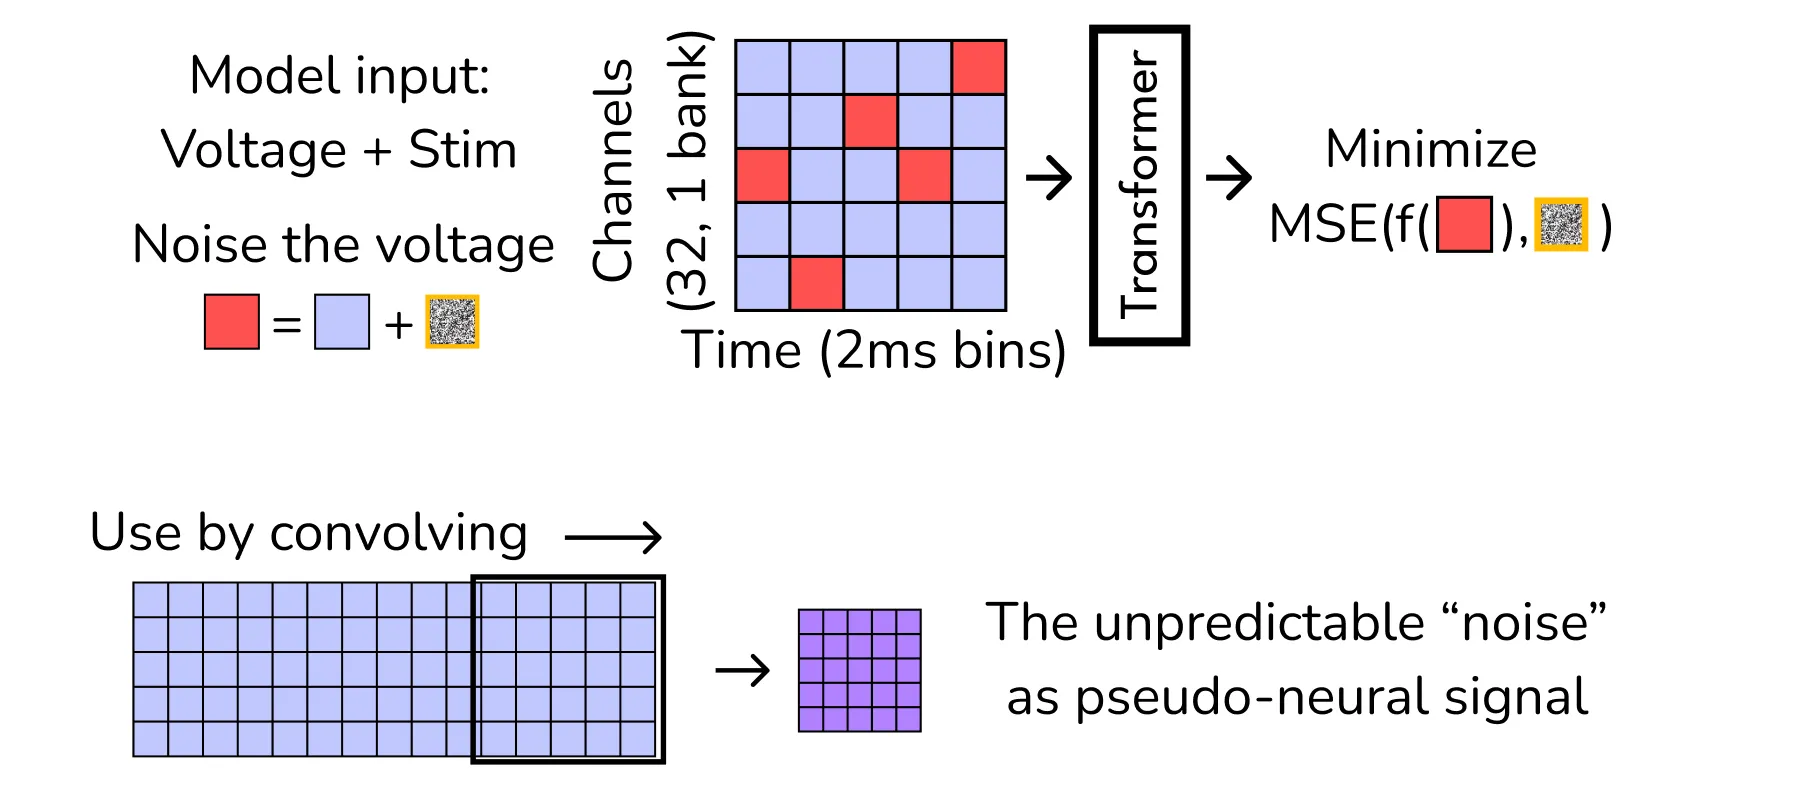
\includegraphics[width=0.5\linewidth]{ch4_delete_schema.png}
  \caption{DELETE method schematic overview.}
  \label{fig:delete_schema}
\end{figure}

\begin{figure}[h]
  \centering
  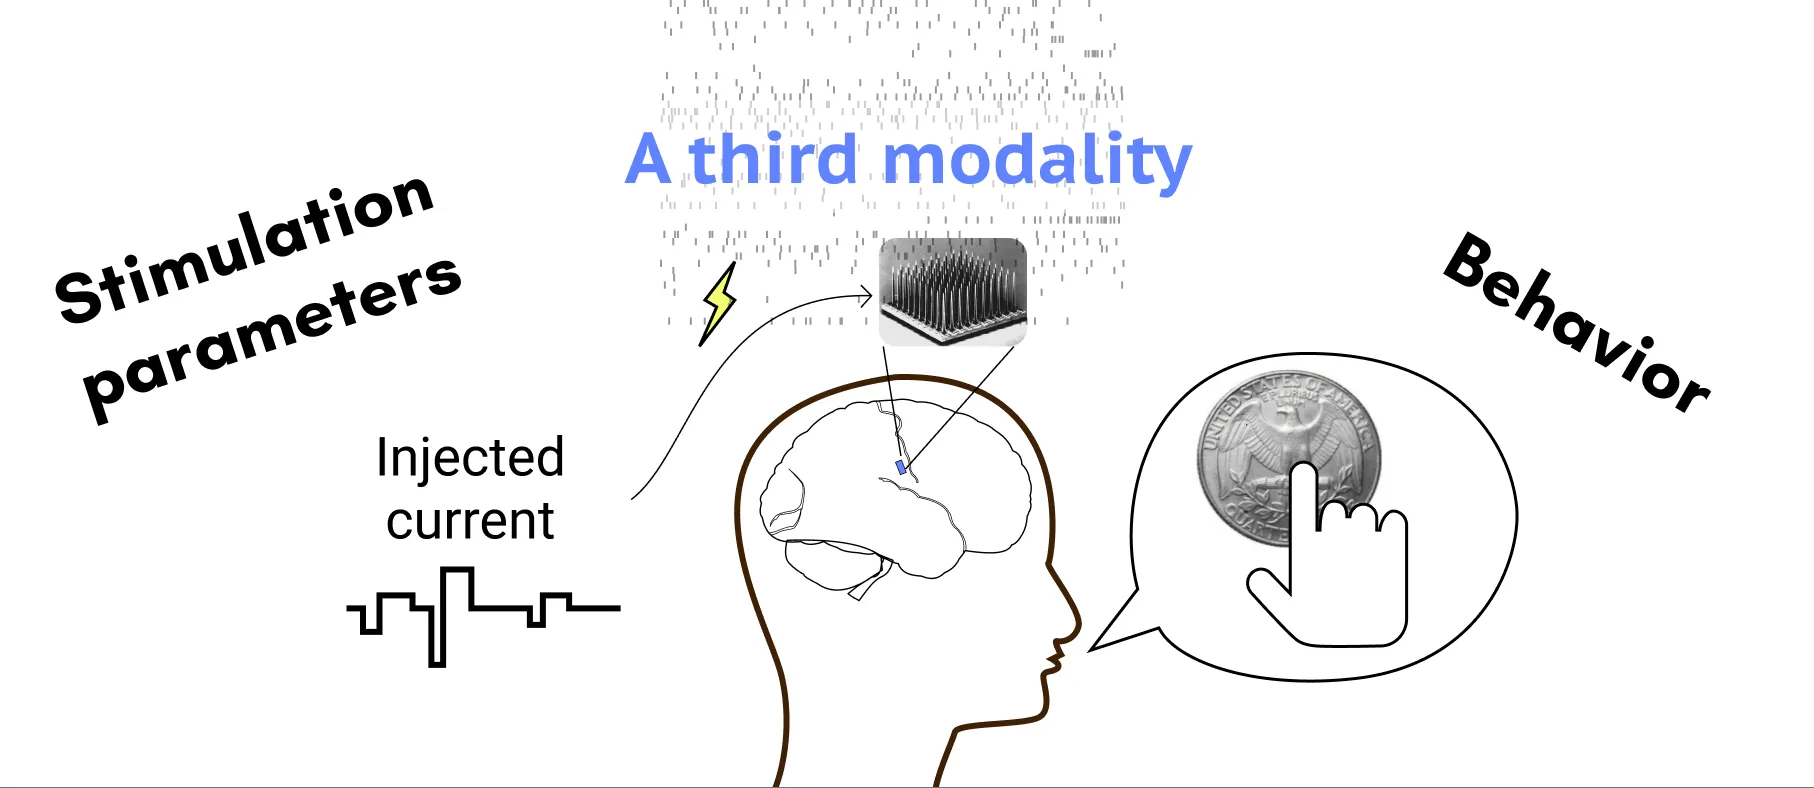
\includegraphics[width=0.5\linewidth]{ch4_third_modality.png}
  \caption{Third modality analysis for ICMS modeling.}
  \label{fig:third_modality}
\end{figure}

\section{Summary and Significance}
Sensory feedback is integral to dexterous control. We decompose the stimulation problem into modeling (i) stimulation$\to$local neural response and (ii) local response$\to$percept. We focus here on (i), introducing DELETE (Denoising Electrical Events with a Transformer Encoder) for artifact removal and using transfer-learning assays to taxonomize ICMS responses across temporal patterns and channels.

\section{Approach}
\subsection*{Recovering the neural response with DELETE}
DELETE reconstructs broadband multichannel activity to estimate and subtract artifacts. Constraints (short windows, point-estimate loss, broad training) reduce the risk of erasing spikes. We benchmark DELETE against PCA/linear baselines and analyze as a generic denoiser on non-ICMS data.

\begin{figure}[h]
  \centering
  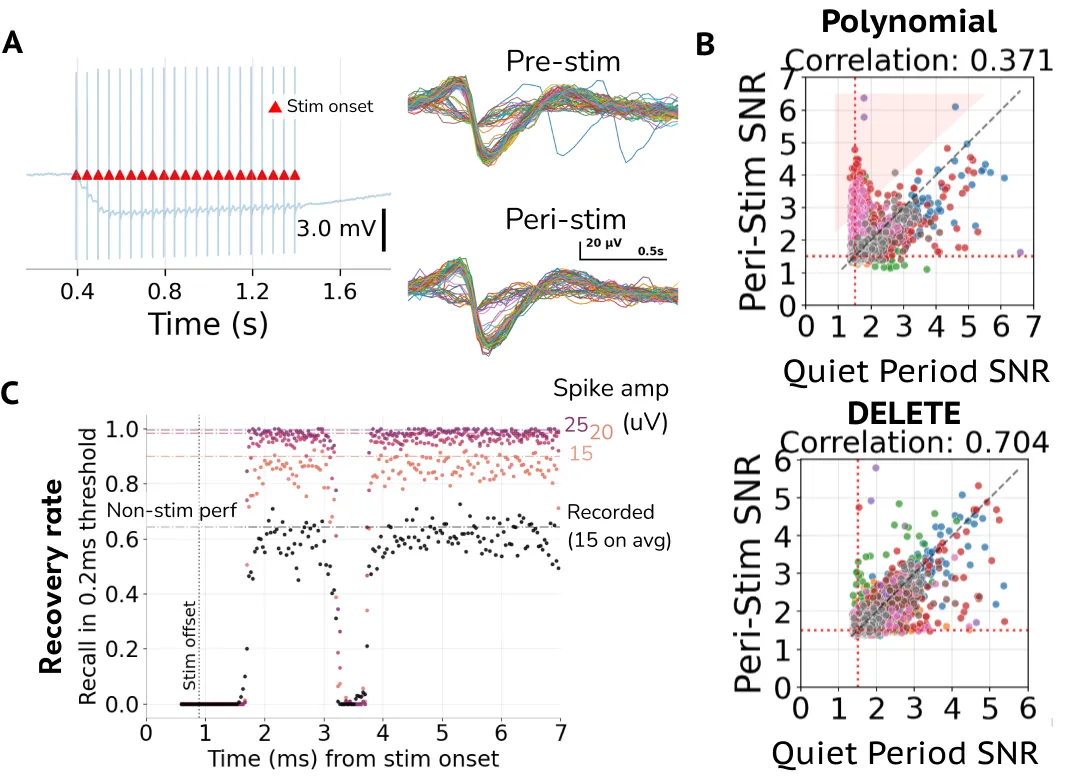
\includegraphics[width=0.5\linewidth]{ch4_delete_peristim.png}
  \caption{A. Left: A sample broadband recording from a channel during a stimulation trial. The displayed channel is on the electrode array that is stimulated. Right: Spike waveforms recovered from the broadband activity both prior to stimulation onset and in the artifacted peri-stimulation period. B. To summarize waveform recovery, we compute channel SNR as a ratio of peak waveform amplitude against background noise amplitude. The color of each dot indicates the physical array the channel is on. We expect physiological waveform SNRs to be conserved through stimulation, so high correlation of quiet period and peri-stim SNR provides a heuristic for good de-artifacting. Dashed red lines indicate the 4.5x background noise threshold we use to determine spike presence. C. We evaluate model sensitivity by injecting synthetic spikes into the broadband activity and evaluating whether they are recovered. The colored curves differ in the precise waveform injected, which were either recorded and extracted from the data or simulated. Horizontal lines indicate the noise ceiling computed as the recovery rate of spikes injected outside of stimulation periods.}
  \label{fig:delete_peristim}
\end{figure}

\subsection*{Taxonomizing passive ICMS responses}
We collect single- and multi-channel passive ICMS datasets including random-amplitude Poisson (RAP) and fixed-train stimuli, and use RNN/Transformer models to test generalization across time patterns, channels, and days.

\begin{figure}[h]
  \centering
  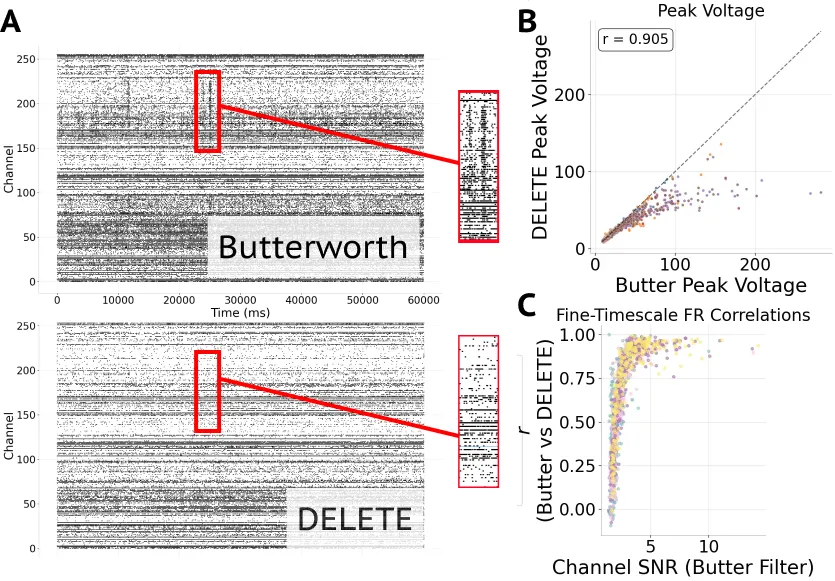
\includegraphics[width=0.5\linewidth]{ch4_delete_generic.png}
  \caption{A. Top: Butteworth filter extracted spiking activity from a minute of resting state recordings. Inset shows putative movement-induced artifact. Bottom: The same data pre-filtered by DELETE, inset no longer shows correlated firing across channels. B. Peak voltages of waveforms extracted by DELETE and a standard Butterworth filter are compared. There is high correlation, but DELETE peaks saturate by 100uV. C. Firing rates are determined by convolving a 50ms Gaussian kernel against Butterworth or DELETE filtered spiking activity. These per-channel firing rates are correlated across a number of different channels and datasets. Color of dots indicate datasets. High SNR channels correlate well.}
  \label{fig:delete_generic}
\end{figure}

\begin{figure}[h]
  \centering
  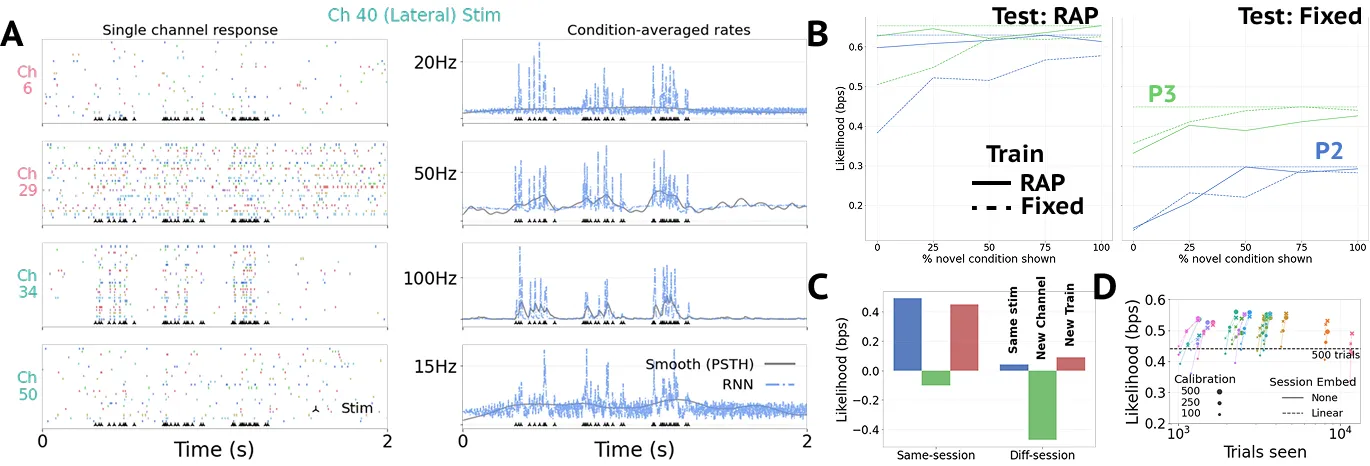
\includegraphics[width=0.5\linewidth]{ch4_icms_taxonomy.png}
  \caption{A. Example raster plots to stimulation on a single channel (40). Modulated responses are visible both on the stimulated array (bottom two rows) and another sensory array (top two rows). Firing rates as inferred by computing PSTH and RNN models are given on the right. B. Example analysis testing generalization of RNN models to novel single channel stimulation trains. In these plots, models are first trained on either random amplitude Possion (RAP) or fixed frequency and amplitude trains (Fixed). They are then gradually exposed to increasing levels (\% novel condition shown) of a new set of ICMS again from either RAP or fixed stimuli (Test condition). The flat dotted line marks the max performance achieved by any in-distribution model. The closer the other curves are to this flat line, the better the model's generalization to new stimuli. C. Here, we train one model on one type of RAP ICMS and assess its generalization to 3 stimulation conditions from either the same or different experimental session. D. We conduct a brief scaled pretraining analysis. We vary the pretraining scale (Trials seen) and subsequent fine-tuning scale (Calibration), and evaluate on a new session. Session identity is either not modeled (Session Embed None) or modeled with a linear readin layer (Linear). The reference line shows session performance using only 500 calibration trials from the evaluation dataset. Most pretrained models exceed this level, suggesting positive transfer.}
  \label{fig:icms_taxonomy}
\end{figure}

\section{Results \& Remaining Work}
DELETE outperforms baselines for peri-stim recovery and preserves high-SNR spike statistics on non-ICMS data. ICMS taxonomy suggests temporal-pattern generalization within-channel is good (RAP$\to$RAP), but cross-channel transfer is weak; multiday models benefit from increased training data but can plateau or regress with RNNs, motivating NDT-style multisession models. Remaining work: finalize DELETE benchmarking suite; ground recovered response statistics physiologically; expand taxonomy across participants/areas or toward inverse-modeling/percept decoding.

% =========================
% Schedule
% =========================
\chapter{Schedule}
I began my doctoral research with a stimulation focus (Aim 3), but put it on hiatus to study how we might aggregate neural datasets (Aim 1). My remaining schedule begins with data collection for NDT-control experiments (Aim 2). As those experiments wind down I expect to be able to focus on writing those results up while running analysis and writeup for Aim 3. Note I expect Aim 3 to produce two publications, one on the artifact removal work and one on the ICMS response taxonomy work.

\begin{figure}[h]
  \centering
  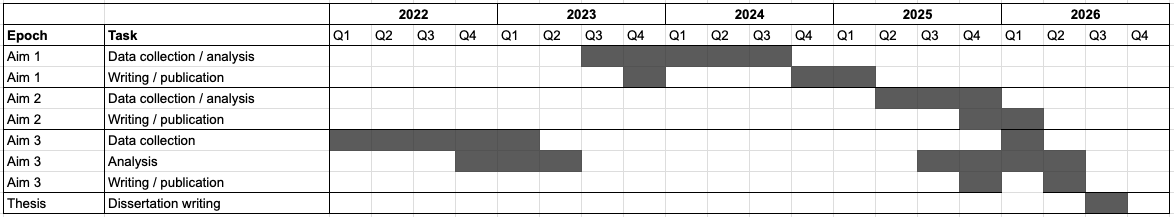
\includegraphics[width=1.0\linewidth]{ch5_schedule_gantt.png}
  \caption{Gantt chart overview of project priorities throughout the PhD.}
  \label{fig:schedule}
\end{figure}

% =========================
% References
% =========================
\cleardoublepage
\printbibliography

\end{document}
